\documentclass[border=6pt]{standalone}
\usepackage{tikz}
\usetikzlibrary{arrows.meta,positioning,shapes.geometric,calc}
\begin{document}
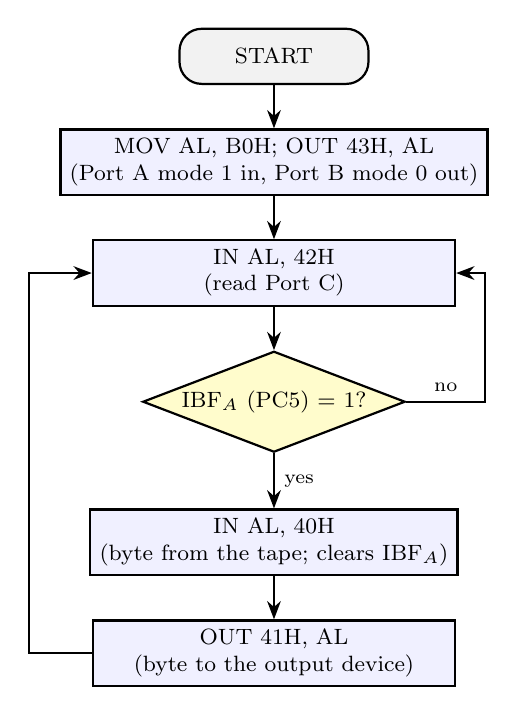
\begin{tikzpicture}[>=Stealth,font=\small,node distance=0.55cm,
 term/.style={draw,thick,rounded corners=8pt,fill=gray!10,minimum width=2.4cm,minimum height=0.7cm,font=\footnotesize},
 proc/.style={draw,thick,fill=blue!6,minimum width=4.6cm,minimum height=0.8cm,align=center,font=\footnotesize},
 dec/.style={draw,thick,diamond,aspect=2.6,fill=yellow!20,align=center,font=\footnotesize,inner sep=1pt}]
\node[term] (s) {START};
\node[proc,below=of s] (init) {MOV AL, B0H; OUT 43H, AL\\(Port A mode 1 in, Port B mode 0 out)};
\node[proc,below=of init] (rdc) {IN AL, 42H\\(read Port C)};
\node[dec,below=of rdc] (ibf) {IBF$_A$ (PC5) = 1?};
\node[proc,below=0.7cm of ibf] (rda) {IN AL, 40H\\(byte from the tape; clears IBF$_A$)};
\node[proc,below=of rda] (wrb) {OUT 41H, AL\\(byte to the output device)};
\draw[->,thick] (s) -- (init);
\draw[->,thick] (init) -- (rdc);
\draw[->,thick] (rdc) -- (ibf);
\draw[->,thick] (ibf) -- (rda) node[midway,right,font=\scriptsize]{yes};
\draw[->,thick] (rda) -- (wrb);
\draw[->,thick] (ibf.east) -- ++(1.0,0) node[pos=0.5,above,font=\scriptsize]{no} |- (rdc.east);
\draw[->,thick] (wrb.west) -- ++(-0.8,0) |- ($(rdc.west)+(0,0)$);
\end{tikzpicture}
\end{document}
